%-------------------------
% Resume in Latex
% Author : Jake Gutierrez
% Based off of: https://github.com/sb2nov/resume
% License : MIT
%------------------------

\documentclass[letterpaper,12t]{article}

\usepackage{latexsym}
\usepackage[empty]{fullpage}
\usepackage{titlesec}
\usepackage{marvosym}
\usepackage[usenames,dvipsnames]{color}
\usepackage{verbatim}
\usepackage{enumitem}
% \usepackage[hidelinks]{hyperref}
\usepackage[colorlinks=true, urlcolor=blue, linkcolor=black]{hyperref}
\usepackage{fancyhdr}
\usepackage[english]{babel}
\usepackage{tabularx}
\input{glyphtounicode}
\usepackage{ragged2e}

\usepackage{graphicx}
\graphicspath{ {../images/} }

%----------FONT OPTIONS----------
% sans-serif
\usepackage[sfdefault]{FiraSans}
% \usepackage[sfdefault]{roboto}
% \usepackage[sfdefault]{noto-sans}
% \usepackage[default]{sourcesanspro}

% serif
% \usepackage{CormorantGaramond}
\usepackage{charter}

\usepackage[T1]{fontenc}

\renewcommand{\normalsize}{\fontsize{11}{14}\selectfont}

\usepackage{ifthen}

\pagestyle{fancy}
\fancyhf{} % clear all header and footer fields
\fancyfoot{}
\renewcommand{\headrulewidth}{0pt}
\renewcommand{\footrulewidth}{0pt}

% Adjust margins
\addtolength{\oddsidemargin}{-0.5in}
\addtolength{\evensidemargin}{-0.5in}
\addtolength{\textwidth}{1in}
\addtolength{\topmargin}{-.5in}
\addtolength{\textheight}{1.0in}

\urlstyle{same}

\raggedbottom
\raggedright
\setlength{\tabcolsep}{0in}

% Sections formatting
\titleformat{\section}{
  \vspace{-4pt}\scshape\raggedright\large
}{}{0em}{}[\color{black}\titlerule \vspace{-5pt}]

% Ensure that generate pdf is machine readable/ATS parsable
\pdfgentounicode=1

%-------------------------
% Custom commands
\newcommand{\resumeItem}[1]{
  \item \small \justifying #1 \vspace{-2pt}
}



\newcommand{\resumeSubheadingFull}[4]{
  \vspace{-2pt}\item
    \begin{tabular*}{0.97\textwidth}[t]{l@{\extracolsep{\fill}}r}
      \textbf{#1} & #2 \\ 
      \textit{\small#3} & \textit{\small #4} \\ 
    \end{tabular*}\vspace{-7pt}
}

\newcommand{\resumeSubheadingSimple}[2]{
  \vspace{-2pt}\item
    \begin{tabular*}{0.97\textwidth}[t]{l@{\extracolsep{\fill}}r}
      \textbf{#1} & #2 \\
    \end{tabular*}\vspace{-7pt}
}

\newcommand{\resumeSubheading}[4]{%
  \if\relax\detokenize{#3}\relax
    \resumeSubheadingSimple{#1}{#2}%
  \else
    \resumeSubheadingFull{#1}{#2}{#3}{#4}%
  \fi
}

\newcommand{\resumeSubSubheading}[2]{
    \item
    \begin{tabular*}{0.97\textwidth}{l@{\extracolsep{\fill}}r}
      \textit{\small#1} & \textit{\small #2} \\ 
    \end{tabular*}\vspace{-7pt}
}

\newcommand{\resumeSubHeading}[2]{
    \item
    \begin{tabular*}{0.97\textwidth}{l@{\extracolsep{\fill}}r}
      \small#1 & #2 \\ 
    \end{tabular*}\vspace{-7pt}
}

\newcommand{\resumeSubItem}[1]{\resumeItem{#1}\vspace{-4pt}}

\renewcommand\labelitemii{$\vcenter{\hbox{\tiny$\bullet$}}$}

\newcommand{\resumeSubHeadingListStart}{\begin{itemize}[leftmargin=0.15in, label={}]}
\newcommand{\resumeSubHeadingListEnd}{\end{itemize}}
\newcommand{\resumeItemListStart}{\begin{itemize}}
\newcommand{\resumeItemListEnd}{\end{itemize}\vspace{-5pt}}

%-------------------------------------------
%%%%%%  RESUME STARTS HERE  %%%%%%%%%%%%%%%%%%%%%%%%%%%%


\begin{document}

%----------HEADING----------
% \begin{tabular*}{\textwidth}{l@{\extracolsep{\fill}}r}
%   \textbf{\href{http://sourabhbajaj.com/}{\Large Sourabh Bajaj}} & Email : \href{mailto:sourabh@sourabhbajaj.com}{sourabh@sourabhbajaj.com}\\
%   \href{http://sourabhbajaj.com/}{http://www.sourabhbajaj.com} & Mobile : +1-123-456-7890 \\
% \end{tabular*}

\begin{center}
    \begin{minipage}[c]{0.17\textwidth}
        \centering
        \setlength{\fboxsep}{0.1pt}
        \setlength{\fboxrule}{2pt}
        \fbox{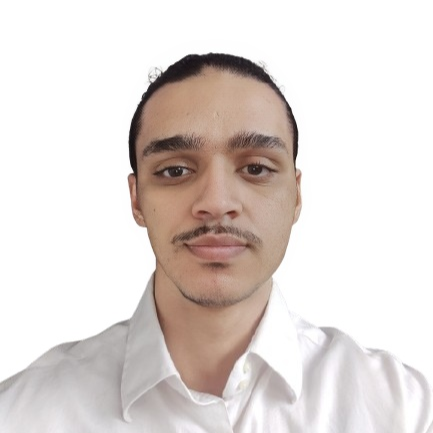
\includegraphics[width=.95\linewidth]{picture.png}}
    \end{minipage}
    \hfill
    \begin{minipage}[c]{0.8\textwidth}
        \textbf{\LARGE \scshape Moncef Bousselat}
        \vspace{3pt}
    
        \textbf{\large \scshape Cloud \& AI Engineer}
        \vspace{5pt}

        \begin{minipage}{\textwidth}
            \justifying \small \noindent
            Graduate in Cloud Computing and holding a Master's in Data and AI, seeking a
            Cloud \& AI role to apply my technical expertise and interdisciplinary 
            skills developed through my academic and professional journey.
        \end{minipage}

        \vspace{5pt}
        
        \raggedright \small 
        % \underline{Contact:}\\
        Nancy, France $|$ 
        \small +33753542166 $|$ 
        \href{mailto:a.m.bousselat@gmail.com@gmail.com}{\underline{a.m.bousselat@gmail.com}} $|$
        \href{https://www.linkedin.com/in/moncefbousselat/}{\underline{linkedin.com/in/moncefbousselat}}
        % \\

        % \underline{Links:}\\
        \href{https://github.com/Somnef}{\underline{github.com/Somnef}} $|$
        \href{https://www.somnef.com}{\underline{somnef.com}}
    \end{minipage}
\end{center}
    
% \vspace{0.5em}
% \noindent\rule{\linewidth}{0.4pt}


%-----------EDUCATION-----------
\section{Education}
    \resumeSubHeadingListStart
        \resumeSubheading
        {Master in Networking and Cloud Computing}{Sep. 2023 -- Jul. 2025}
        {University of Lorraine $|$ Leeds Beckett University $|$ Lulea Technical University}{Nancy, FR $|$ Leeds, UK $|$ Skelleftea, SE}
            \resumeItemListStart
                \resumeItem{Selected among 2000+ applicants for the Erasmus Mundus scholarship in "Green Networking and Cloud Computing"}
                \resumeItem{Relevant coursework: Cloud Services, Intelligent Systems and Robotics, Internet of Things, Advanced Wireless Networks, System Engineering, QoS and QoE, Data Analysis}
            \resumeItemListEnd
      
        \resumeSubheading
        {Master in Data Science and AI}{Sep. 2018 -- Jul. 2023}
        {National Polytechnic School}{Algiers, Algeria}
            \resumeItemListStart
                \resumeItem{Ranked in the top 10\% of prepatory school students nationwide, selected through a national competitive exam}
                \resumeItem{Relevant coursework: Advanced Databases, Probability and Statistics, Multivariate Data Analysis, Machine \& Deep Learning, NLP, Blockchain, Cloud Computing}
            \resumeItemListEnd
  \resumeSubHeadingListEnd


%-----------EXPERIENCE-----------
\section{Professional Experience}
    \resumeSubHeadingListStart
        \resumeSubheading
        {Cloud Engineer -- Intern}{Dec. 2024 -- Jul. 2025}
        {University of Lorraine}{Nancy, France}
            \resumeItemListStart
                \resumeItem{Built a decentralized Self-Sovereign Identity (SSI) system with Hyperledger Indy for secure information sharing in the cloud}
                \resumeItem{Deployed the control agents on AWS with Docker (ECS) and benchmarking of system performance}
            \resumeItemListEnd

        \resumeSubheading
        {Full-Stack Developer -- Intern}{Jan. 2023 -- Jul. 2023}
        {Schlumberger}{Algiers, Algeria}
            \resumeItemListStart
                \resumeItem{Developed a REST API to log 1000+ transactions/day on a Hyperledger Fabric private blockchain}
                \resumeItem{Built a Flask/Vue Dockerized app to manage the blockchain and deployed it on ECS, reducing penalty costs by 75\%}
            \resumeItemListEnd

        \resumeSubheading
        {Data and AI Engineer - Intern}{Oct. 2022 -- Jan. 2023}
        {Ericsson}{Algiers, Algeria}
            \resumeItemListStart
                \resumeItem{Trained a YOLO model to help field workers identify devices, with 85\%+ accuracy}
                \resumeItem{Built a PyTorch autoencoder for image denoising; 99\% accuracy on MNIST}
            \resumeItemListEnd
    

        \resumeSubheading
        {Data Analyst - Intern}{May 2022 -- Jul. 2022}
        {BH Advisory}{Algiers, Algeria}
            \resumeItemListStart
                \resumeItem{Monitored the construction materials market to spot price and stock trends}
                \resumeItem{Built web scrapers and displayed data on a VueJS dashboard}
            \resumeItemListEnd
    
    \resumeSubHeadingListEnd


%-----------PROJECTS-----------
\section{Projects}
    \resumeSubHeadingListStart

        \resumeSubheading
        {Auto-scaling Infrastructure on AWS with Terraform}{Jan. 2025}
        {\href{https://github.com/Somnef/d7001d-lab4}{\underline{View on GitHub}}}{}
            \resumeItemListStart
                \resumeItem{Designed JADE agents to simulate DDoS attacks on EC2, generating 20000+ instances per minute}
                \resumeItem{Implemented an auto-scalable infrastructure resilient to attacks via Terraform}
                \resumeItem{Developed VueJS dashboard integrating AWS SDK for CloudWatch metrics monitoring}
            \resumeItemListEnd

        \resumeSubheading
        {Fault Tolerance in Kubernetes Orchestrated Systems}{Nov. 2024}
        {\href{https://github.com/Somnef/kubernetes-fault-tolerance}{\underline{View on GitHub}}}{}
            \resumeItemListStart
                \resumeItem{Deployed a Python app on Kubernetes cluster with an HPA for load balancing}
                \resumeItem{Load-tested the system using cURL - Achieved 99.9\% uptime}
                \resumeItem{Real-time resource monitoring with Prometheus and Grafana}
            \resumeItemListEnd

        \resumeSubheading
        {Machine Learning for Drinking Water Quality Evaluation}{May 2024}
        {\href{https://github.com/Somnef/dl-water-quality}{\underline{View on GitHub}}}{}
        {}{}
            \resumeItemListStart
                \resumeItem{Used chemical features to classify water as drinkable or not through ML and DL models, reaching 90\% accuracy}
            \resumeItemListEnd

        \resumeSubheading
        {Benchmarking GPU Energy Consumption for Deep Learning}{Apr. 2024}
        {\href{https://github.com/Somnef/gpu-profiling-for-dl}{\underline{View on GitHub}}}{}
            \resumeItemListStart
                \resumeItem{Built a GPU profiler to test 25+ hyperparameter setups for energy use}
                \resumeItem{Found an optimal setup with 20\% energy savings and top accuracy}
            \resumeItemListEnd
    
        \resumeSubheading
        {Room Recommender Based on IoT}{Nov. 2023}
        {\href{https://github.com/Somnef/iot_project_app}{\underline{View on GitHub}}}{}
            \resumeItemListStart
                \resumeItem{Deployed an app on AWS EC2 to collect IoT data (temperature, noise) and store it on MongoDB}
                \resumeItem{Developed a decision algorithm to recommend rooms based on user preferences}
            \resumeItemListEnd

        \resumeSubheading
        {Business Game}{May 2022}
        {}{}
            \resumeItemListStart
                \resumeItem{Led student dev team to build and improve a market simulation game}
                \resumeItem{Optimized traffic for 12 teams, handling 1000+ req/min on local servers}
            \resumeItemListEnd

        \resumeSubheading
            {NEAT Algorithm Applied to Video Games}{Oct. 2022}
            {\href{https://github.com/Somnef/snake_neat_ai}{\underline{View on GitHub}}}{}
                \resumeItemListStart
                    \resumeItem{Rebuilt Flappy Bird and Snake in Pygame with matching gameplay}
                    \resumeItem{Used NEAT to evolve agents with unsupervised training and outperformed all tested human players}
                \resumeItemListEnd

        \resumeSubheading
        {Wildfire 3D Simulator}{Dec. 2021}
        {\href{https://github.com/Somnef/semi-empirical-wildfire-simulation}{\underline{View on GitHub}} $|$ \href{https://www.researchgate.net/publication/354678516_Applying_semi-empirical_simulation_of_wildfire_on_real_world_satellite_imagery_data}{\underline{Read on ResearchGate}}}{}
            \resumeItemListStart
                \resumeItem{Segmented Google Earth Engine satellite imagery with k-means clustering for terrain mapping}
                \resumeItem{Rebuilt the 3D landscape for a 100km² forest area and simulated wildfire spread using a semi-empirical cellular automata}
            \resumeItemListEnd
    

        \resumeSubheading
        {Focus AI}{Nov. 2021}
        {\href{https://github.com/Somnef/focus-monitor-ai}{\underline{View on GitHub}}}{}
            \resumeItemListStart
            \resumeItem{Optimized a deep learning face tracker to detect loss of focus in real time using Mediapipe}
            \resumeItem{User tests showed up to 50\% boost in focus and productivity}
            \resumeItemListEnd
    

        \resumeSubheading
        {Online Store Scraper}{Apr. 2021}
        {\href{https://github.com/Somnef/CdiscountScrapper}{\underline{View on GitHub}}}{}
            \resumeItemListStart
                \resumeItem{Built scrapers for Amazon, CDiscount, and Materiel.net with price tracking}
                \resumeItem{Enabled multi-site comparison with 15\% average cost savings on products}
            \resumeItemListEnd
    
      
    \resumeSubHeadingListEnd



%
%-----------AWARDS-----------
\section{Awards \& Certifications}
    \begin{itemize}[leftmargin=0.15in, label={}]
        \item{
            \textbf{Certifications}{: AWS Certified Solutions Architect Associate}\\
            \textbf{Awards}{: 1st Place - Arctic Challenge (Sweden, 2024), 2nd Place - Google DevFest Hackathon 21 (Algeria, 2021)}\\
        }
    \end{itemize}

%-----------SKILLS-----------
\section{Skills}
    \begin{itemize}[leftmargin=0.15in, label={}]
        \item{
        \textbf{Programming Languages}{: Python, C/C++, Java, PHP/SQL, JavaScript/TypeScript, BASH} \\
        \textbf{Tools and Technologies}{: NumPy, Pandas, Matplotlib, Seaborn, PyTorch, Scikit-learn, Tensorflow, Anaconda, AWS (certified), Terraform, Docker, Kubernetes, Git, CI/CD, Monitoring (Prometheus, Grafana)} \\
        \textbf{Languages}{: English (C2), French (C2), Arabic (Native), Swedish (Basic)} \\
        }
    \end{itemize}

%-------------------------------------------
\end{document}
